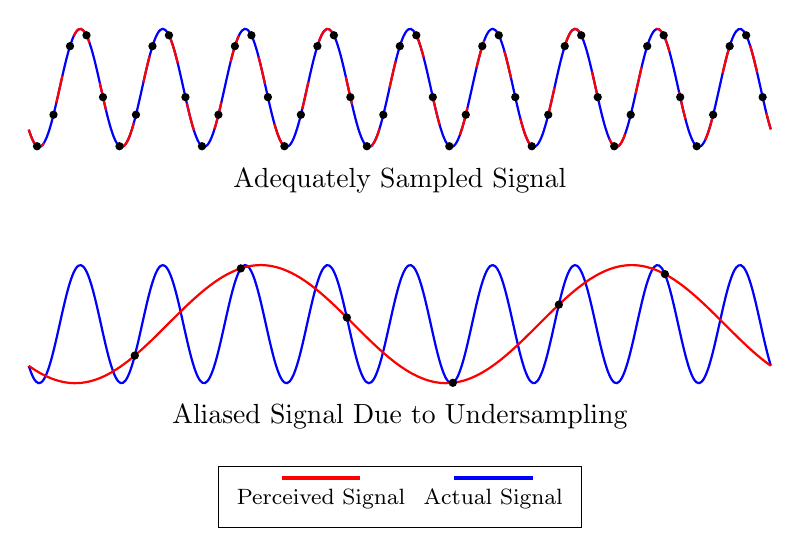
\begin{tikzpicture}[scale=1.5]

% Above Signal
\draw[
domain=0:2*pi, 
samples=300,
smooth,
variable=\x,
blue,
thick,
shift={(0, 2)}
] plot ({\x},{sin((9*\x - 3*pi/4) r)/2});

% Above Perceived
\draw[
domain=0:2*pi, 
samples=300,
smooth,
variable=\x,
red,
thick,
dash pattern={on 10pt off 15pt},
shift={(0, 2)}
] plot ({\x},{sin((9*\x - 3*pi/4) r)/2});

% Scatter Adequate Samples
\foreach \i in {1,...,45} {
    \pgfmathsetmacro\xsamp{2*pi*(\i-0.5)/45}
    \pgfmathsetmacro\ysamp{sin((9*\xsamp - 3*pi/4) r)/2}
    \fill (\xsamp, \ysamp + 2) circle (1pt);
}

% Above Text
\node[
anchor=north, 
] at (pi, 1.4) {Adequately Sampled Signal};


% Below Signal
\draw[
domain=0:2*pi, 
samples=300,
smooth,
variable=\x,
blue,
thick
] plot ({\x},{sin((9*\x - 3*pi/4) r)/2});

% Below Perceived
\draw[
domain=0:2*pi, 
samples=100,
smooth,
variable=\x,
red,
thick
] plot ({\x},{sin((2*\x - 3*pi/4) r)/2});

% Scatter Aliasing Samples
\foreach \i in {1,...,6} {
    \pgfmathsetmacro\xsamp{2*pi*\i/7}
    \pgfmathsetmacro\ysamp{sin((9*\xsamp - 3*pi/4) r)/2}
    \fill (\xsamp, \ysamp) circle (1pt);
}

% Below Text
\node[
anchor=north, 
] at (pi, -0.6) {Aliased Signal Due to Undersampling};


% Legend
\tikzset{
    legend entry/.pic={
        \draw[pic actions, line width=1.5pt] (-0.5, 0) -- (0.5, 0);
    }
}
\matrix [draw, below] at (pi, -1.2) {
    \pic[red]{legend entry}; &  \pic[blue]{legend entry}; \\
    \node[font=\footnotesize] {Perceived Signal}; &  \node[font=\footnotesize] {Actual Signal}; \\
};

\end{tikzpicture}